    %------------------第五章---------------------------
\newpage
\section{超声波接近传感器实物制作与检测}
\subsection{超声波接近传感器实物制作}
\subsubsection{超声波接近传感器的实物焊接}
在完成硬件部分和软件部分的设计之后,就将进行元器件采购、打板、实物焊接制作。如图\ref{PCB实物焊接图}为焊接完成后的实物图。
\begin{figure}[!h]
	\centering
	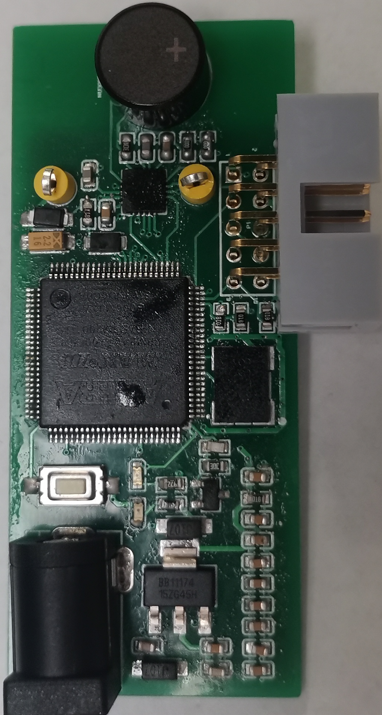
\includegraphics[width=8cm,angle=-90]{figure/physical map.png}
	\caption{PCB实物焊接图}
	\label{PCB实物焊接图}
\end{figure}\par
在焊接开始之前,为方便后续的焊接,首先要确定各个元器件的焊接顺序。根据焊接经验,本设计选取的焊接顺序为CPLD芯片->TUSS4470超声驱动芯片->其它贴片器。在确定好焊接顺序后,就可以开始正式焊接。首先清理电路板,然后用电烙铁焊接好CPLD芯片,并确保各引脚间没有存在虚焊、粘结等情况;焊接完成CPLD芯片后进行驱动芯片的焊接,首先在电路板上涂上焊锡膏,将芯片正确摆放,用热风枪加热焊锡膏使其融化,并轻轻按压芯片使焊盘上锡,最后再用电烙铁将粘结的引脚分离;其它的贴片器件贼按照涂焊锡膏、摆放器件、用热风枪加热的步骤来完成焊接;插件使用电烙铁来焊接。\par
在完成焊接后,还需检查焊点是否光滑、平整、没有短路和冷焊等问题,使用显微镜或放大镜检查焊点的质量。检查无误后,再用洗板水清洗电路板,去除在焊接过程中多余的松香、锡膏等杂物。清洗完成后,就可以通电进行程序的调试。

\subsubsection{超声波接近传感器的调试}
通过示波器对各引脚输出的波形进行检测,然后修改程序,直至每个引脚可以输出正常波形,以下为传感器正常工作时各引脚输出的波形。\par
\begin{figure}[!h]
	\centering
	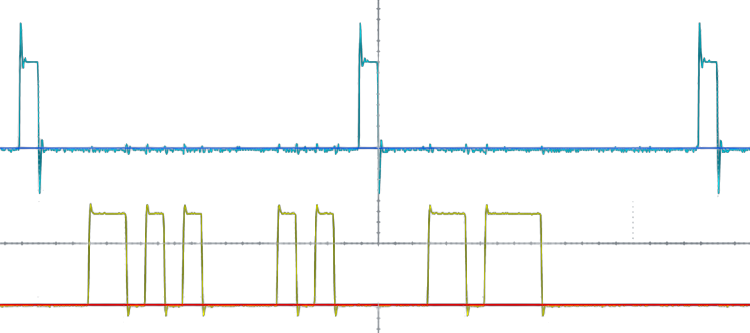
\includegraphics[width=8cm,height=3.5cm]{figure/debug waveform1.png}
	\caption{SPI发送数据波形图}
	\label{SPI发送数据波形图}
\end{figure}\par
如图\ref{SPI发送数据波形图},为采样率100MHz时示波器采集的波形,上方蓝色的为NSS端口的波形,下方黄色的为MOSI端口向驱动芯片发送的配置数据。可以看到,当NSS信号拉低时,MCU开始发送数据,等待一帧数据发送完成后,NSS拉高,并且在下一帧数据发送前,NSS会再次拉低,以实现低-高-低的过程。本设计的程序可以实现连续发送10帧配置数据的功能。
\begin{figure}[!h]
	\centering
	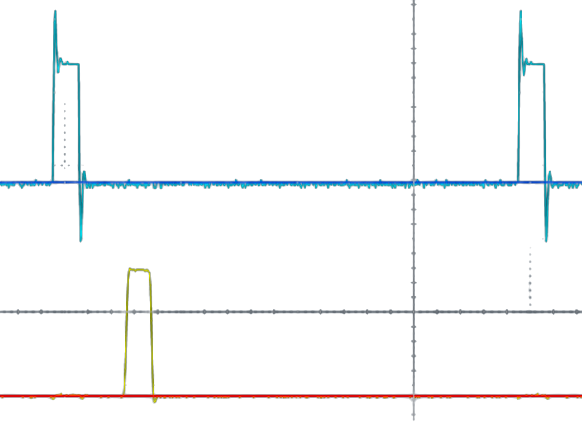
\includegraphics[width=8cm,height=3.5cm]{figure/debug waveform2.png}
	\caption{SPI接收数据波形图}
	\label{SPI接收数据波形图}
\end{figure}\par
图\ref{SPI接收数据波形图}为SPI接收数据的波形图,上方蓝色的波形为NSS端口发送的信号,下方黄色的为MISO端口接收的波形信号。当每次NSS信号拉低时,超声驱动芯片会向MCU返回数据,返回数据的结构如图\ref{SPI数据结构图1}和表\ref{芯片状态表}所示,当传感器正常工作时,只有VDRV\_READY状态位为1,其余位都为0。
\newpage
\begin{figure}[!h]
	\centering
	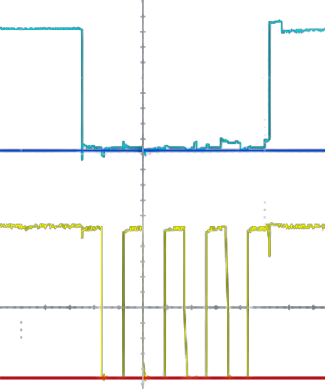
\includegraphics[width=8cm,height=3.5cm]{figure/debug waveform9.png}
	\caption{io1、io2引脚波形图}
	\label{io1、io2引脚波形图}
\end{figure}\par
如图\ref{io1、io2引脚波形图}所示,上方波形为io1端口信号,下方波形为io2端口信号,两引脚按照IO模式3产生信号,当io1引脚信号拉低时,io2开始产生波形,直到产生指定脉冲数波形后,io1拉高,停止产生波形。

\begin{figure}[!h]
	\centering
	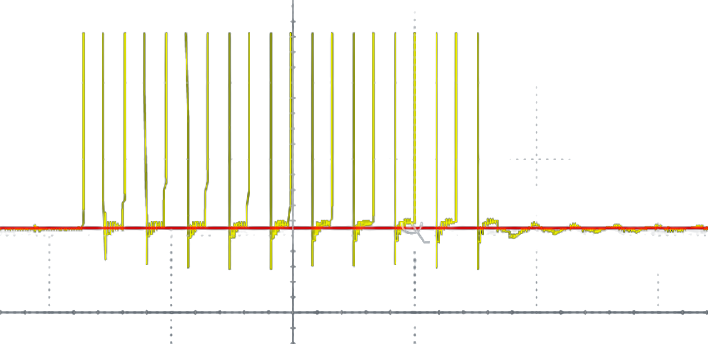
\includegraphics[width=8cm,height=3.5cm]{figure/debug waveform3.png}
	\caption{超声探头波形图1}
	\label{超声探头波形图1}
\end{figure}\par
图\ref{超声探头波形图1}为OUTA和OUTB引脚输出的波形,采样频率50MHz,可以看到,探头发出了10个周期频率为300kHz的脉冲波。
\begin{figure}[!h]
	\centering
	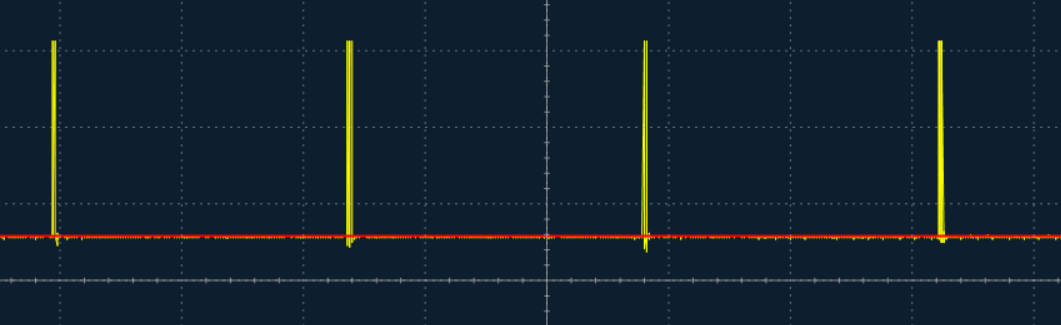
\includegraphics[width=8cm]{figure/debug waveform4.png}
	\caption{超声探头波形图2}
	\label{超声探头波形图2}
\end{figure}\par
图\ref{超声探头波形图2}为示波器采样率10MHz时采集到的波形,超声探头连续的发送波形,以10个脉冲为发送周期,每过2.4ms完成一次脉冲的发送。
\newpage
\begin{figure}[!h]
	\centering
	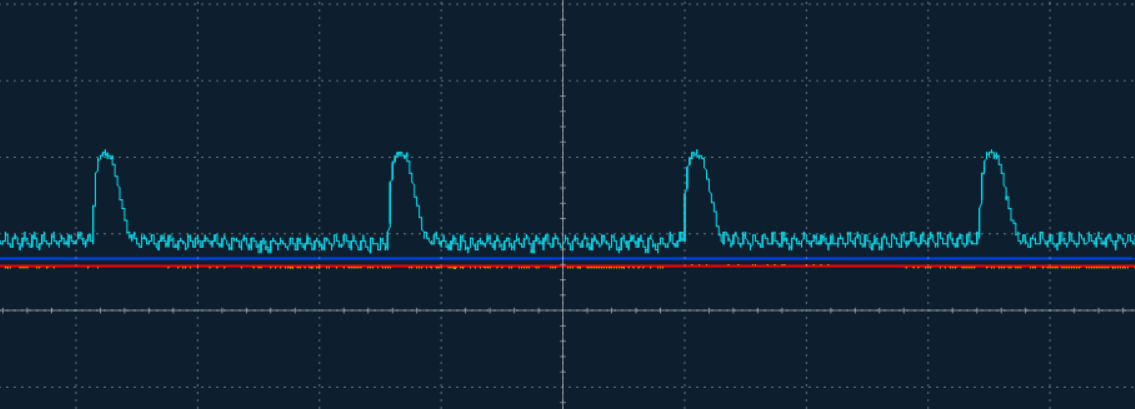
\includegraphics[width=8cm,height=3.5cm]{figure/debug waveform5.png}
	\caption{VOUT引脚波形图(无物体遮挡)}
	\label{VOUT引脚波形图(无物体遮挡)}
\end{figure}\par

图\ref{VOUT引脚波形图(无物体遮挡)}为无物体遮挡的情况下,VOUT引脚输出的波形,采样频率为1MHz。第一个波峰为探头发出脉冲信号时所引起的干扰,在设计检测程序时需要屏蔽该段的信号,经测量,该段信号的持续时间约为发射脉冲后的0.5ms。
\begin{figure}[!h]
	\centering
	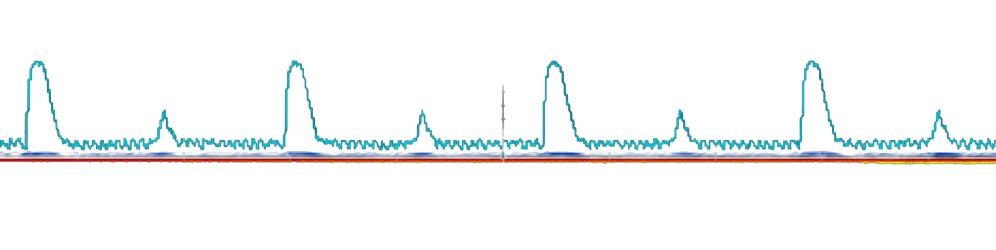
\includegraphics[width=8cm,height=3.5cm]{figure/debug waveform6.png}
	\caption{VOUT引脚波形图(有物体遮挡)}
	\label{VOUT引脚波形图(有物体遮挡)}
\end{figure}\par
图\ref{VOUT引脚波形图(有物体遮挡)}为有物体遮挡时VOUT引脚的输出波形,采样频率为1MHz。当有物体遮挡时,发射的10个脉冲波遇到物体后会进行反射,重新被探头所接收。经过芯片的放大解调处理,形成第二个峰值较低的波峰。
\begin{figure}[!h]
	\centering
	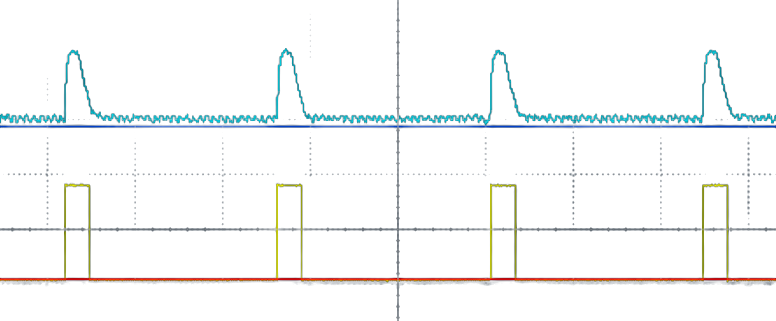
\includegraphics[width=8cm,height=3.5cm]{figure/debug waveform7.png}
	\caption{OUT4引脚波形图(无物体遮挡)}
	\label{OUT4引脚波形图(无物体遮挡)}
\end{figure}\par
图\ref{OUT4引脚波形图(无物体遮挡)}为OUT4引脚的输出波形,采样频率为1MHz。根据芯片手册中所介绍内容,我们不难知道,当VOUT引脚的电压值超过所设定的阈值时,OUT4引脚就会拉高。上图所示波形VOUT的阈值设置为0.9V,当VOUT形成第一个波峰时,电压值超过0.9V的频段OUT4也会拉高。
\newpage
\begin{figure}[!h]
	\centering
	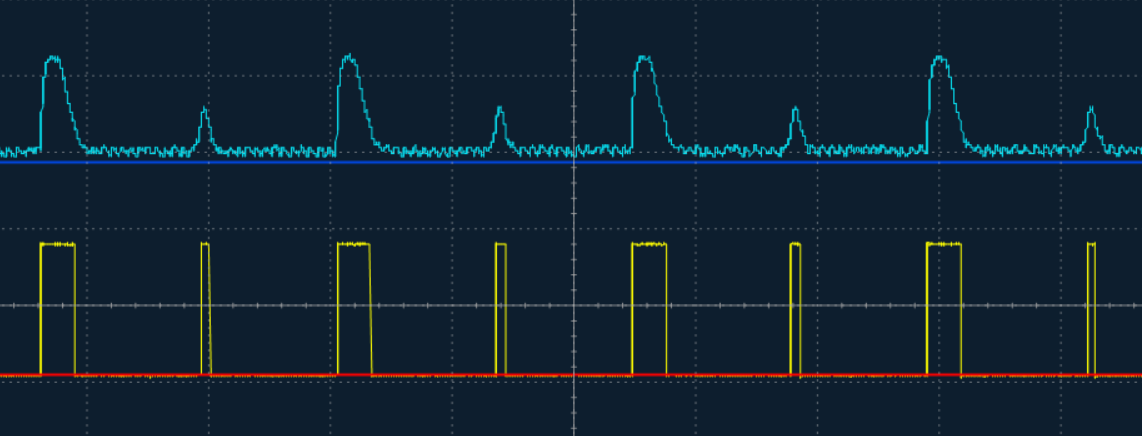
\includegraphics[width=8cm,height=3.5cm]{figure/debug wave form8.png}
	\caption{OUT4引脚波形图(有物体遮挡)}
	\label{OUT4引脚波形图(有物体遮挡)}
\end{figure}\par
图\ref{OUT4引脚波形图(有物体遮挡)}为有物体遮挡时OUT4引脚输出的波形,采样频率为1MHz。当有物体遮挡时,VOUT处理回波产生第二个波峰,而这第二个波峰才是检测所需要用到的有效信号。在这个频段中,VOUT电压值超过所设定的阈值,OUT4第二次拉高,该信号将作为检测物体的重要触发事件。为屏蔽OUT4的第一次拉高信号,在MAIN模块中需要延时一段时间,跳过第一个信号后再开始进行检测,此时只会检测到OUT4的第二个拉高信号,检测有效。



\subsection{超声波接近传感器实验}
\subsubsection{实验器材}
在本设计的实验测试当中,选用虚拟示波器作为调试仪器,如图\ref{虚拟示波器}所示。配合功能强大的上位机软件,该示波器不仅有基础功能,还具有显示灵活、精度高、波形数据可存储等优点,十分适合本设计的试验调试。\par
其它实验材料如图\ref{其他实验器材}所示,包括了直尺、12V直流电源供电插头、100mm$\times$100mm的测试板材。

\begin{figure}[ht]
	\centering
	\subfloat[虚拟示波器]{
		\begin{minipage}[b]{0.5\textwidth}
			\centering
			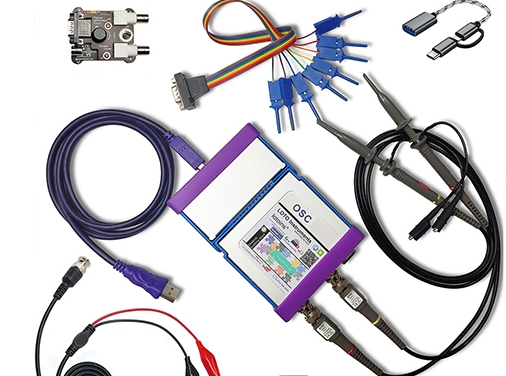
\includegraphics[height=4.5cm]{figure/虚拟示波器.png}
		\end{minipage}
		\label{虚拟示波器}
	}
	\subfloat[其他实验器材]{
		\begin{minipage}[b]{0.5\textwidth}
			\centering
			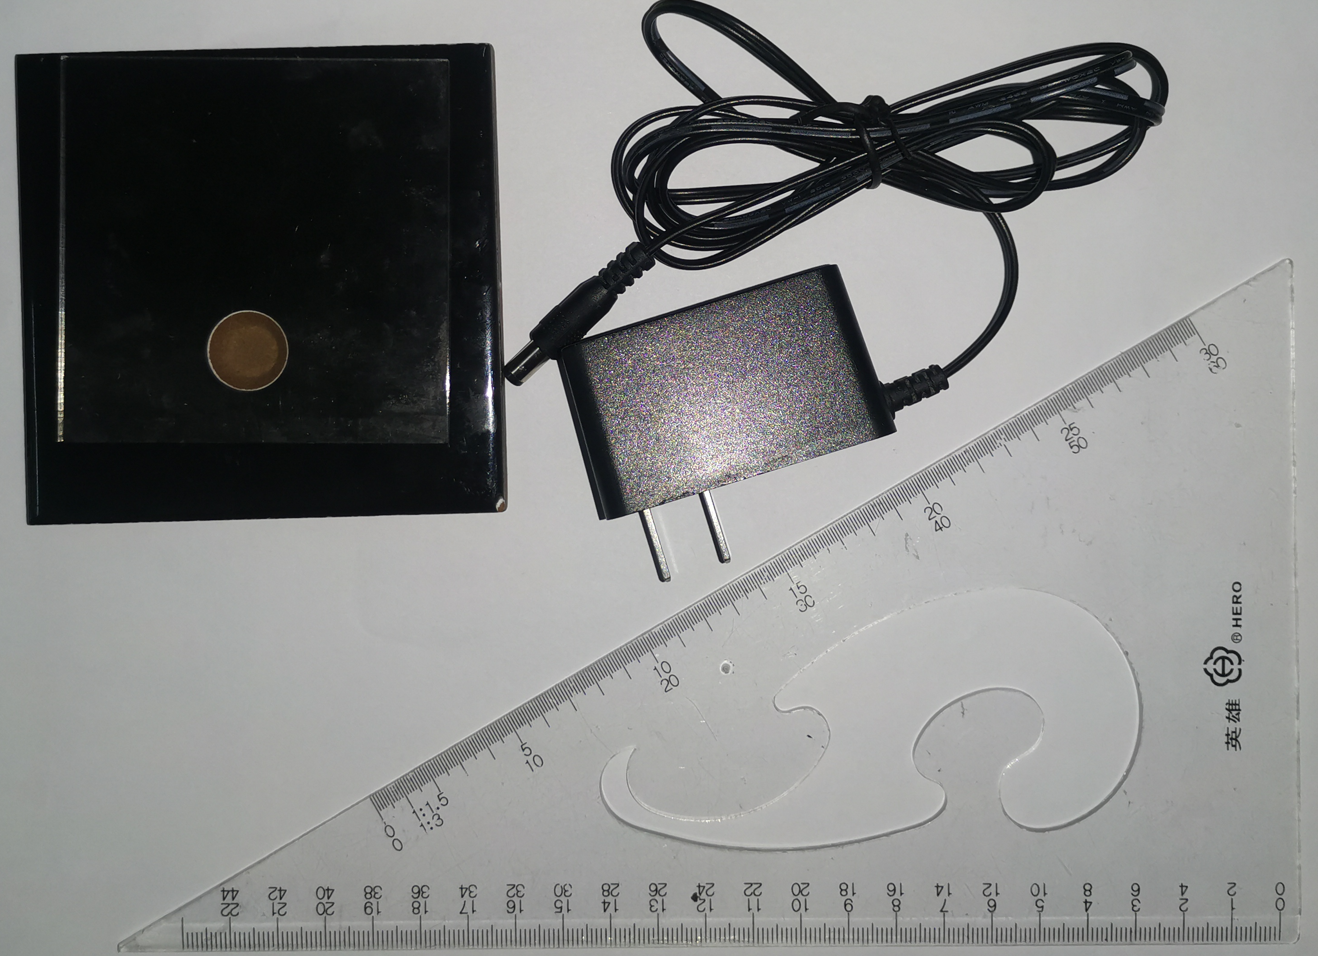
\includegraphics[height=4.5cm]{figure/实验器材图.png}
		\end{minipage}
		\label{其他实验器材}
	}
	\caption{实验器材图}
	\label{实验器材图}
\end{figure}
\subsubsection{超声波接近传感器性能参数测试}
在本设计的实验中,对传感器的各性能参数进行了测试,如表所示,有效检测范围为100mm-200mm,传感器精度为1mm,LED检测指示灯刷新的频率为83.3Hz,即每过12ms完成一次检测状态的刷新。
\begin{table}[!h]
	\centering
	\caption{性能参数表}
	
	\begin{GDUTtable}{\textwidth}{Y Y Y}
		\textbf{参数名 }& \textbf{参数值} &\textbf{单位}    \\ 
		\hline
		检测范围    &   100-200 & $mm$  \\ 
		检测精度 &  1 & $mm$  \\
		检测周期 &  2.4 &$ms$  \\      
		
	\end{GDUTtable}   
\end{table}


\subsubsection{超声波接近传感器检测策略测试}
对传感器检测策略的可行性进行测试,验证检测策略的必要性。检测物体的材料为亚克力板,检测距离为150mm,将检测物体分为干扰处理与未干扰处理两组。进行的干扰处理操作为,将检测物体表面用粉笔灰覆盖,以达到干扰回波的作用。在检测周期不变的情况下,调整检测次数阈值,观察应对干扰的效果,未进行干扰处理、进行干扰处理的实验结果分别如表\ref{未进行干扰处理测试}、\ref{进行干扰处理测试}所示。\par
\begin{table}[!h]
	\centering
	\caption{未进行干扰处理测试}
	
	\begin{GDUTtable}{\textwidth}{Y Y Y}
		\textbf{检测次数 }& \textbf{检测阈值} & \textbf{是否检测到物体}    \\ 
		\hline
		6 &  6 & 是  \\
		6 &  5 & 是  \\
		6 &  4 & 是  \\    
		6 &  3 & 是  \\    
		6 &  2 & 是  \\
		6 &  1 & 是  \\        
		
	\end{GDUTtable}
	\label{未进行干扰处理测试}    
\end{table}
\begin{table}[!h]
	\centering
	\caption{进行干扰处理测试}
	
	\begin{GDUTtable}{\textwidth}{Y Y Y}
		\textbf{检测次数 }& \textbf{检测阈值} & \textbf{是否检测到物体}    \\ 
		\hline
		6 &  6 & 否  \\
		6 &  5 & 否  \\
		6 &  4 & 否  \\    
		6 &  3 & 否  \\    
		6 &  2 & 是  \\
		6 &  1 & 是  \\        
		
	\end{GDUTtable}
	\label{进行干扰处理测试}    
\end{table}\par
可以看到,在检测物体存在干扰时,可以通过调整检测逻辑来提高传感器的抗干扰性,保证其在各种复杂的应用场景都能正常工作。

\subsubsection{不同材料测试}
将测试物体放置在距离超声波传感器150mm的位置,每次发射脉冲数为8的脉冲,对于不同材料的检测物体进行测试,观察VOUT波形的峰值,测量五次取平均值。实验材料为亚克力板、纸板、陶瓷板、玻璃,实验结果如表所示。
\begin{table}[!h]
	\centering
	\caption{不同材料测试结果}
	\begin{GDUTtable}{\textwidth}{Y Y Y}
		\textbf{材料类型 }& \textbf{VOUT波形峰值} &\textbf{单位}      \\
		\hline
		亚克力板 & 0.79 &V  \\
		纸板 & 0.78 &V \\
		陶瓷板 & 0.79 &V\\
		玻璃 & 0.80 &V\\
	\end{GDUTtable}
\end{table}\par
根据实验结果,我们可以画出各材料对应回波峰值的折线图,如图所示。通过观察图形,我们可以得知,VOUT回波与物体的材质并无太大关系,当检测物体材质改变时,VOUT引脚输出的波形并没有太大的变化,而与反射脉冲波的强度有关。

\subsubsection{不同脉冲数测试}
将检测物体放置在距离超声波传感器150mm的位置,改变每次发送脉冲波的脉冲数,观察VOUT波形峰值的变化情况。\par
实验中取到的脉冲数为3,5,7,9,11,检测物体的材质为亚克力板和陶瓷板,每组实验重复五次取平均值,实验结果如图\ref{不同脉冲数实验结果}所示,
\begin{figure}[!h]
	\centering
	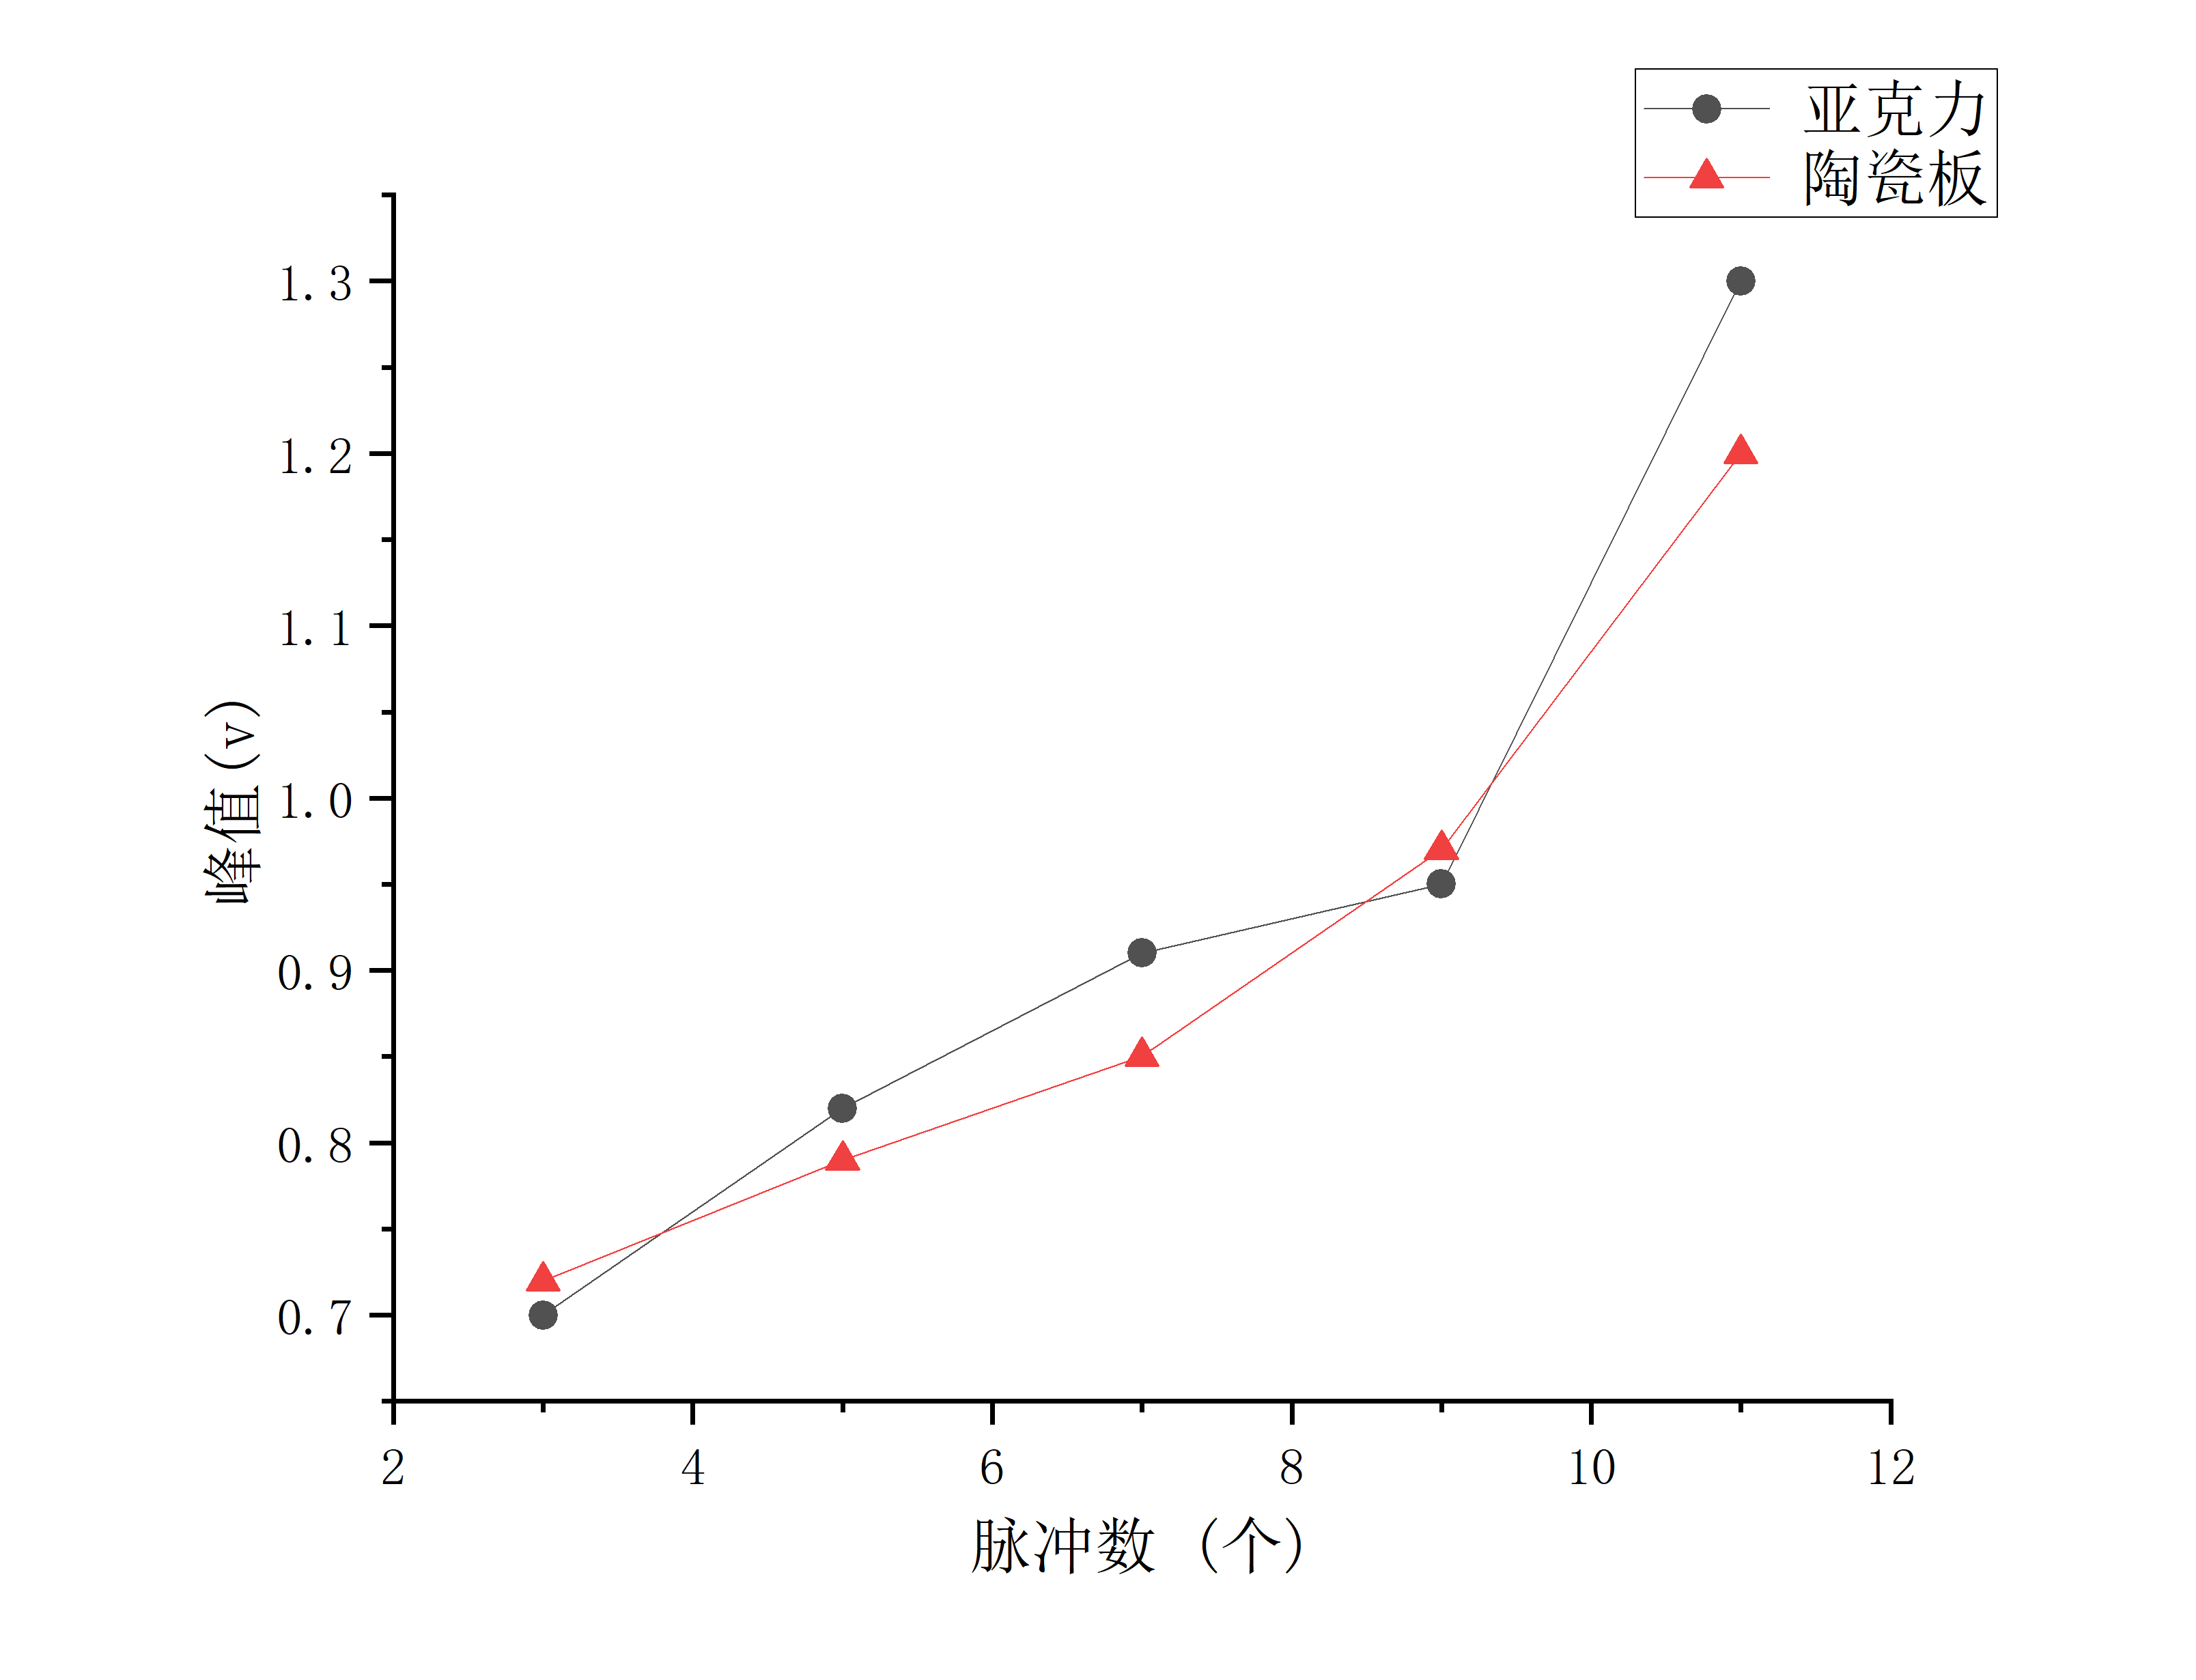
\includegraphics[width=8cm]{figure/G3.png}
	\caption{不同脉冲数实验结果}
	\label{不同脉冲数实验结果}
\end{figure}\par



图中每个数据点都为实验五次取平均值后的结果,可以看到,当每次发射脉冲波的脉冲数越多时,VOUT引脚的峰值就越大。

\subsubsection{不同距离测试}
以亚克力板和陶瓷板作为检测物体,将测试物体放置在距离传感器50mm,100mm,150mm,200mm,250mm的位置,测试其回波信号$t$值的大小,$t$值为波峰距离检测周期起点的时间,实验结果如图所示,图\ref{亚克力板}为亚克力板的实验结果作图,图\ref{陶瓷板}为陶瓷板的实验结果作图。
\begin{figure}[!h]
	\centering
	\subfloat[亚克力板]{
		\begin{minipage}[c]{0.5\textwidth}
			\centering
			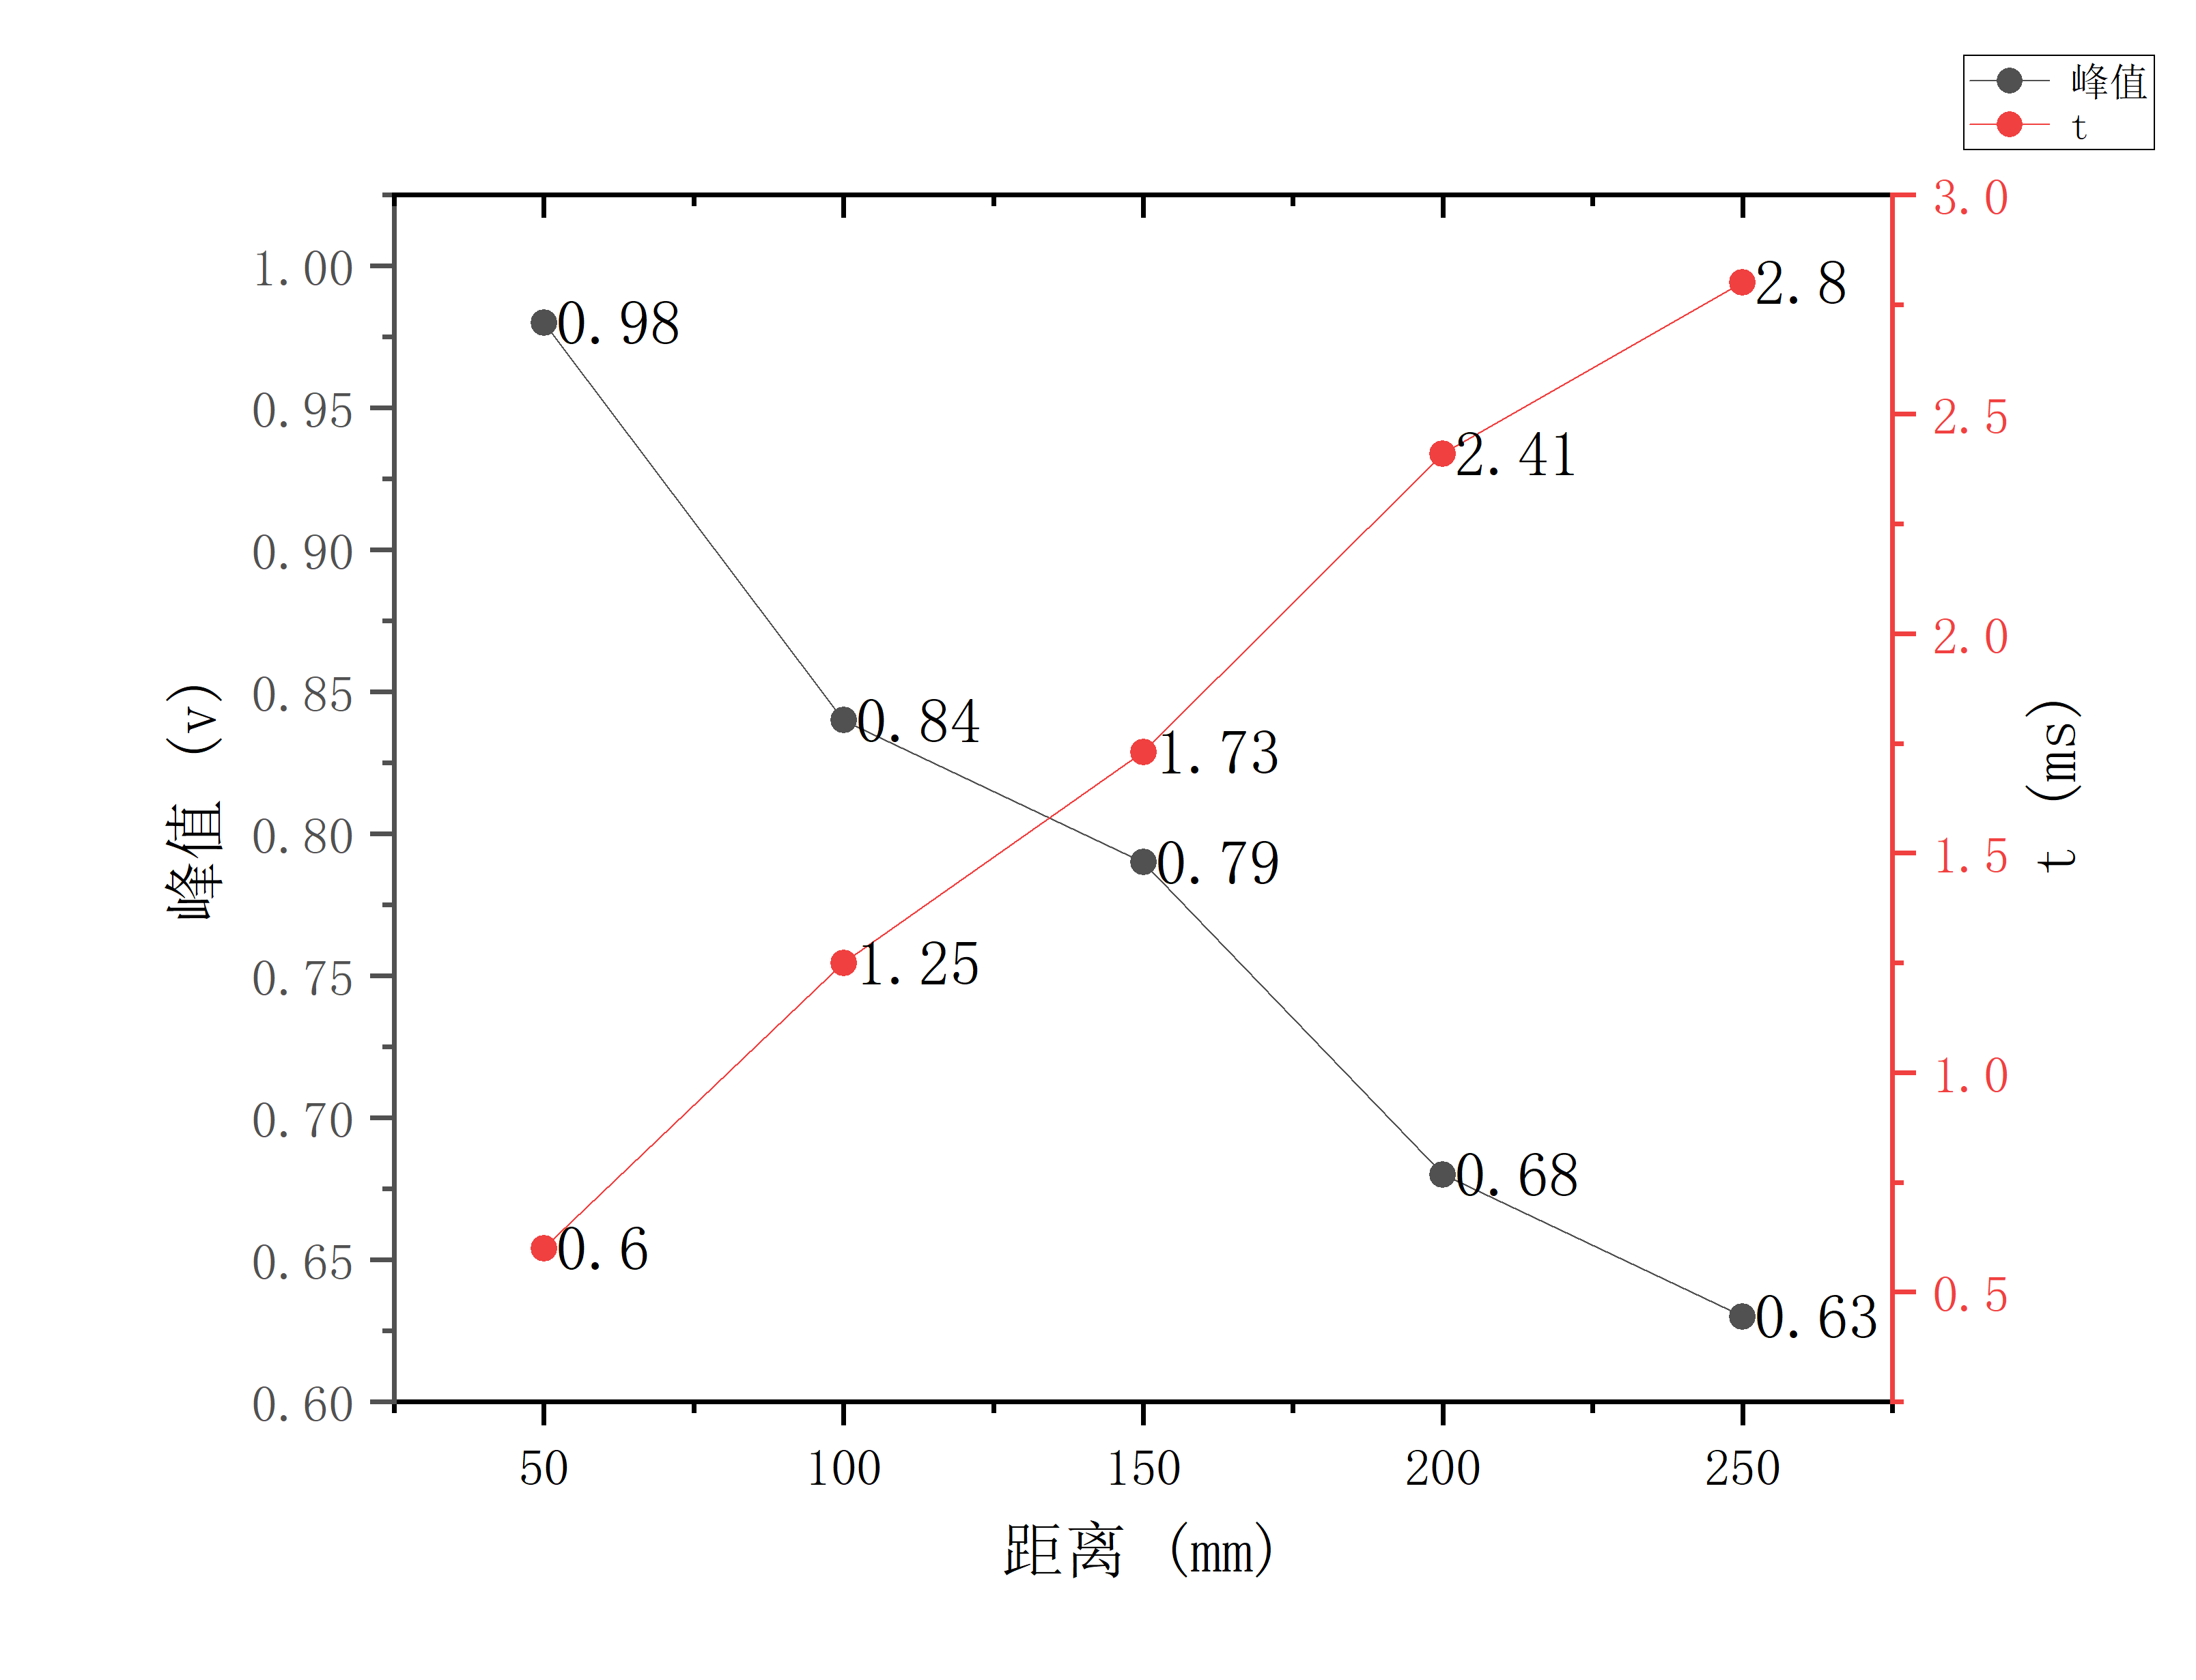
\includegraphics[height=5.5cm]{figure/G1.png}
		\end{minipage}
		\label{亚克力板}
	}
	\subfloat[陶瓷板]{
		\begin{minipage}[c]{0.5\textwidth}
			\centering
			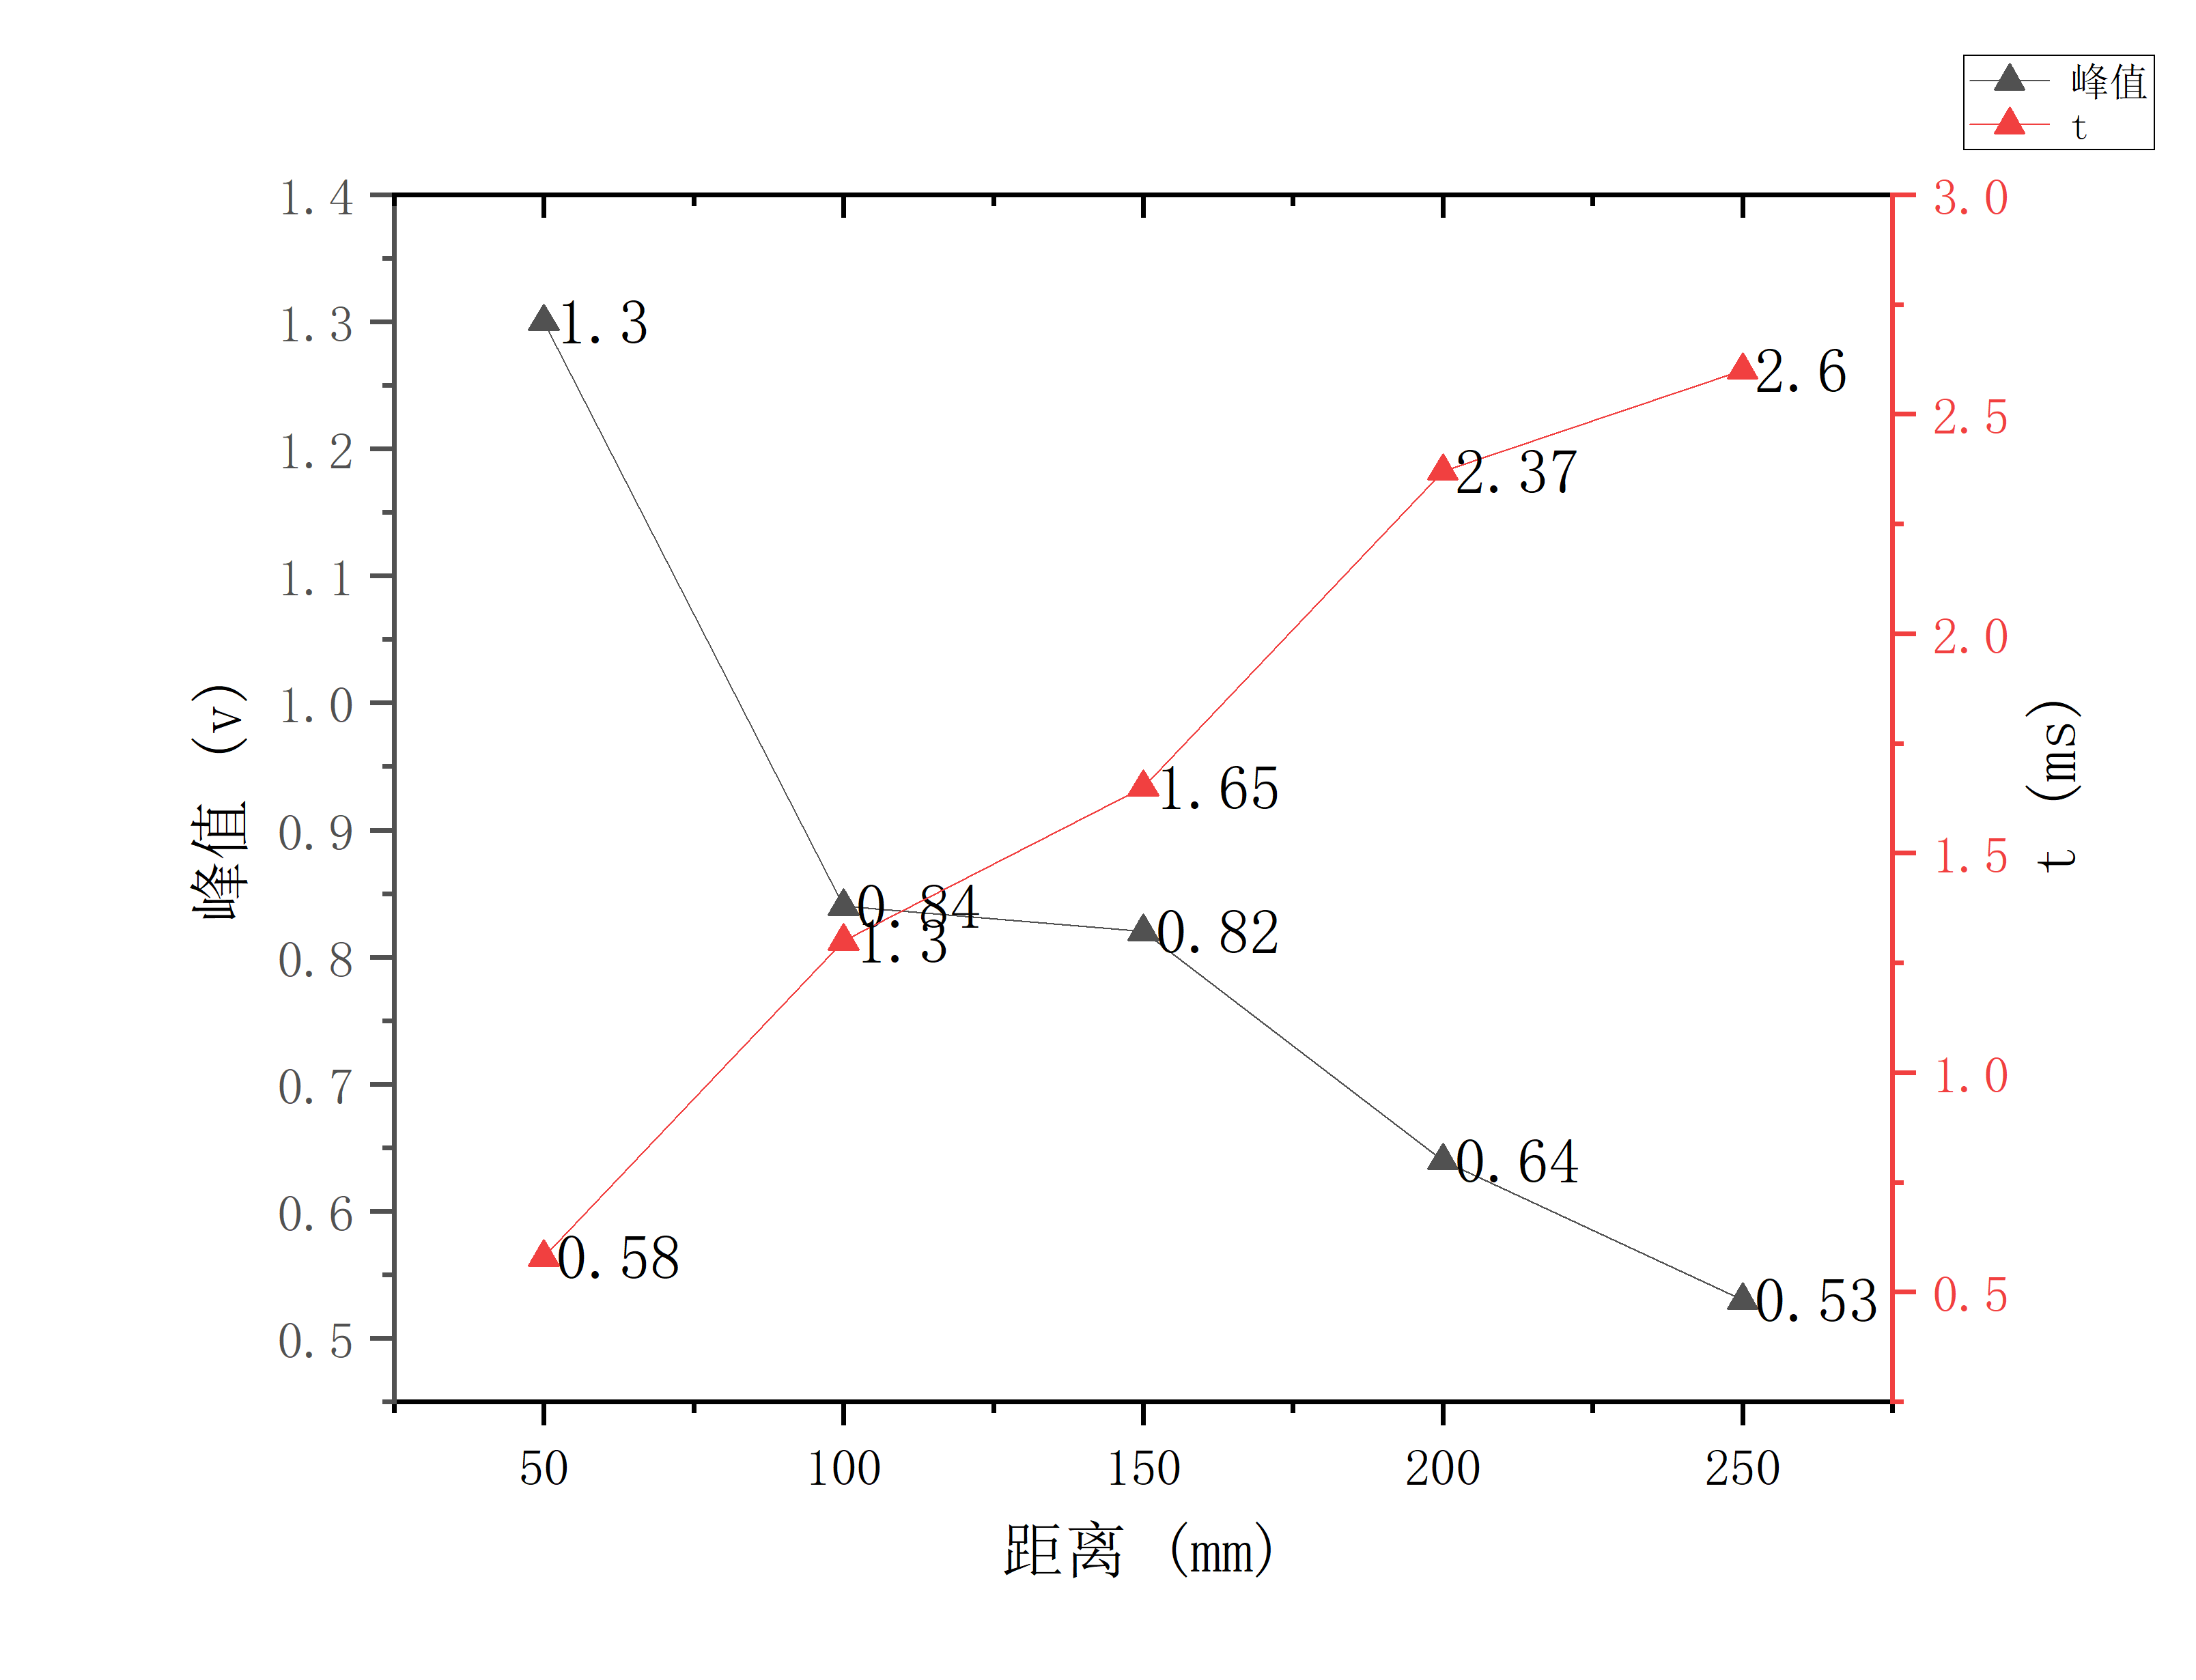
\includegraphics[height=5.5cm]{figure/G2.png}
		\end{minipage}
		\label{陶瓷板}
	}
	\caption{不同距离实验结果}
	\label{不同距离实验结果}
\end{figure}\par
可以看到,当检测距离增加时,VOUT第二个波峰的峰值在不断减小,距离检测起点的时间也在不断增加,与图\ref{VOUT输出}对比,实验结果相近,可以证明传感器脉冲发射与回波接收没有异常。
\subsection{本章小结}
本章首先介绍了超声波接近传感器实物焊接的流程,然后列举了实物调试过程中所记录的波形图,将其与仿真波形进行了比较。然后介绍了实验器材以及五种实验方案的设计,列举了处理后的实验数据,并对实验结果进行初步分析。下一章将对本设计所存在的不足进行总结,并提出对后续的展望。







